\documentclass[tikz,border=12pt]{standalone}
\usepackage{tikz}
\usetikzlibrary{shapes.geometric,arrows.meta,positioning,fit,backgrounds,calc}

\renewcommand{\familydefault}{\sfdefault}
\definecolor{cborder}{HTML}{1E293B}
\definecolor{cbg}{HTML}{F8FAFC}
\definecolor{cbox}{HTML}{FFFFFF}
\definecolor{cblue}{HTML}{1E40AF}
\definecolor{cbluelight}{HTML}{EFF6FF}
\definecolor{cgray}{HTML}{64748B}
\definecolor{cgreen}{HTML}{059669}
\definecolor{cgreenlight}{HTML}{ECFDF5}

\begin{document}
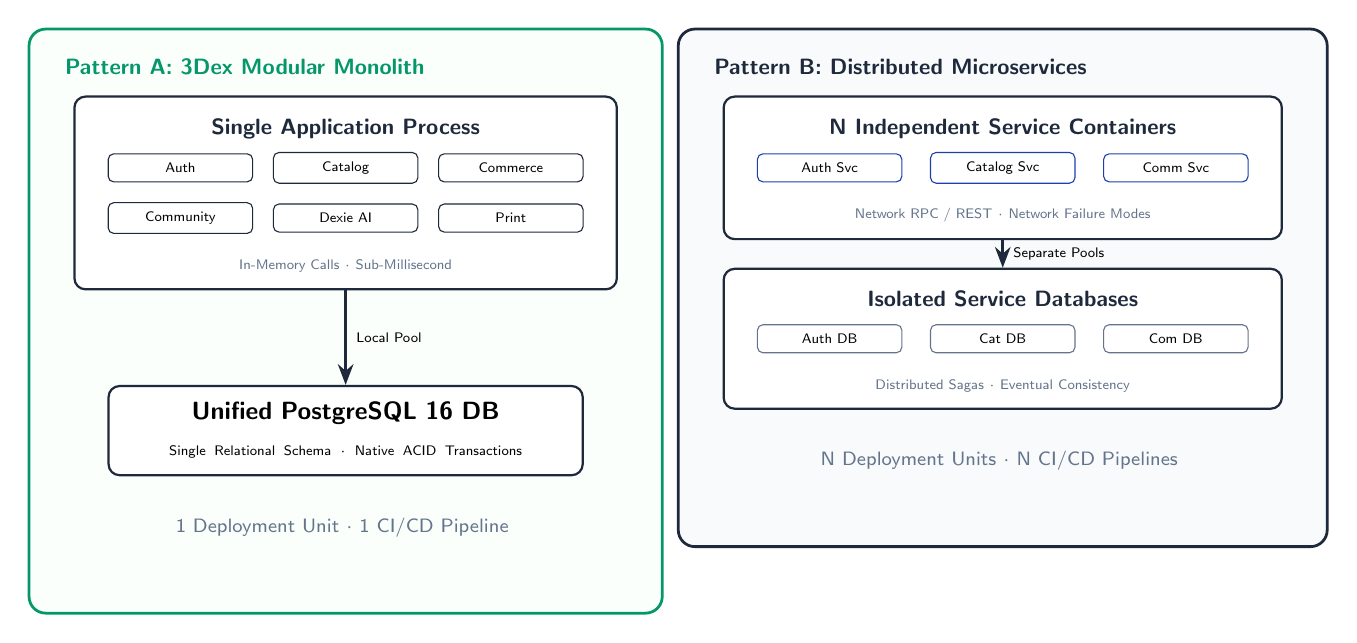
\begin{tikzpicture}[
    font=\small,
    >=Stealth,
    node distance=0.5cm and 0.4cm,
    flow/.style={
        ->,
        line width=1pt,
        draw=cborder
    },
    netflow/.style={
        <->,
        line width=0.8pt,
        draw=cblue,
        dashed
    }
]

    % ================= PANE A: MODULAR MONOLITH =================
    \node[draw=cborder, fill=white, rounded corners=2pt, font=\tiny, text width=1.6cm, align=center] (a1) {Auth};
    \node[draw=cborder, fill=white, rounded corners=2pt, font=\tiny, text width=1.6cm, align=center, right=0.25cm of a1] (a2) {Catalog};
    \node[draw=cborder, fill=white, rounded corners=2pt, font=\tiny, text width=1.6cm, align=center, right=0.25cm of a2] (a3) {Commerce};
    \node[draw=cborder, fill=white, rounded corners=2pt, font=\tiny, text width=1.6cm, align=center, below=0.25cm of a1] (a4) {Community};
    \node[draw=cborder, fill=white, rounded corners=2pt, font=\tiny, text width=1.6cm, align=center, right=0.25cm of a4] (a5) {Dexie AI};
    \node[draw=cborder, fill=white, rounded corners=2pt, font=\tiny, text width=1.6cm, align=center, right=0.25cm of a5] (a6) {Print};

    % Container for Monolith App on main layer with clean border
    \node[draw=cborder, fill=white, rounded corners=4pt, line width=0.8pt,
          fit=(a1) (a2) (a3) (a4) (a5) (a6),
          inner xsep=12pt, inner ysep=20pt] (mono_app) {};

    % Re-stamp modules on top
    \node[draw=cborder, fill=white, rounded corners=2pt, font=\tiny, text width=1.6cm, align=center] at (a1) {Auth};
    \node[draw=cborder, fill=white, rounded corners=2pt, font=\tiny, text width=1.6cm, align=center] at (a2) {Catalog};
    \node[draw=cborder, fill=white, rounded corners=2pt, font=\tiny, text width=1.6cm, align=center] at (a3) {Commerce};
    \node[draw=cborder, fill=white, rounded corners=2pt, font=\tiny, text width=1.6cm, align=center] at (a4) {Community};
    \node[draw=cborder, fill=white, rounded corners=2pt, font=\tiny, text width=1.6cm, align=center] at (a5) {Dexie AI};
    \node[draw=cborder, fill=white, rounded corners=2pt, font=\tiny, text width=1.6cm, align=center] at (a6) {Print};

    \node[anchor=north, font=\bfseries\footnotesize, text=cborder] at (mono_app.north) [yshift=-5pt] {
        Single Application Process
    };
    \node[anchor=south, font=\tiny, text=cgray] at (mono_app.south) [yshift=3pt] {
        In-Memory Calls $\cdot$ Sub-Millisecond
    };

    % Monolith DB
    \node[draw=cborder, fill=white, rounded corners=4pt, line width=0.8pt,
          below=1.2cm of mono_app.south, text width=5.6cm, align=center, inner sep=6pt] (mono_db) {
        \textbf{Unified PostgreSQL 16 DB}\\[2pt]
        \tiny Single Relational Schema $\cdot$ Native ACID Transactions
    };

    \draw[flow] (mono_app.south) -- (mono_db.north) node[midway, right, font=\tiny] {Local Pool};

    \node[below=0.4cm of mono_db, font=\scriptsize, align=center, text=cgray] (lbl_a) {
        1 Deployment Unit $\cdot$ 1 CI/CD Pipeline
    };

    % Pane A Outer Boundary
    \begin{scope}[on background layer]
        \node[draw=cgreen, fill=cgreenlight!25, rounded corners=6pt, line width=1pt,
              fit=(mono_app) (mono_db) (lbl_a),
              inner xsep=16pt, inner ysep=24pt] (pane_a) {};
    \end{scope}

    \node[anchor=north west, font=\bfseries\footnotesize, text=cgreen] at (pane_a.north west) [xshift=10pt, yshift=-8pt] {
        Pattern A: 3Dex Modular Monolith
    };

    % ================= PANE B: MICROSERVICES =================
    \node[draw=cblue, fill=white, rounded corners=2pt, font=\tiny, text width=1.6cm, align=center, right=2.2cm of a3] (b1) {Auth Svc};
    \node[draw=cblue, fill=white, rounded corners=2pt, font=\tiny, text width=1.6cm, align=center, right=0.35cm of b1] (b2) {Catalog Svc};
    \node[draw=cblue, fill=white, rounded corners=2pt, font=\tiny, text width=1.6cm, align=center, right=0.35cm of b2] (b3) {Comm Svc};

    \draw[netflow] (b1) -- (b2);
    \draw[netflow] (b2) -- (b3);

    % Container for Microservices on main layer
    \node[draw=cborder, fill=white, rounded corners=4pt, line width=0.8pt,
          fit=(b1) (b2) (b3),
          inner xsep=12pt, inner ysep=20pt] (micro_apps) {};

    % Re-stamp services on top
    \node[draw=cblue, fill=white, rounded corners=2pt, font=\tiny, text width=1.6cm, align=center] at (b1) {Auth Svc};
    \node[draw=cblue, fill=white, rounded corners=2pt, font=\tiny, text width=1.6cm, align=center] at (b2) {Catalog Svc};
    \node[draw=cblue, fill=white, rounded corners=2pt, font=\tiny, text width=1.6cm, align=center] at (b3) {Comm Svc};

    \node[anchor=north, font=\bfseries\footnotesize, text=cborder] at (micro_apps.north) [yshift=-5pt] {
        N Independent Service Containers
    };
    \node[anchor=south, font=\tiny, text=cgray] at (micro_apps.south) [yshift=3pt] {
        Network RPC / REST $\cdot$ Network Failure Modes
    };

    % Isolated Databases positioned cleanly below micro_apps
    \node[draw=cgray, fill=white, rounded corners=2pt, font=\tiny, text width=1.6cm, align=center, below=1.8cm of b1] (d1) {Auth DB};
    \node[draw=cgray, fill=white, rounded corners=2pt, font=\tiny, text width=1.6cm, align=center, right=0.35cm of d1] (d2) {Cat DB};
    \node[draw=cgray, fill=white, rounded corners=2pt, font=\tiny, text width=1.6cm, align=center, right=0.35cm of d2] (d3) {Com DB};

    \node[draw=cborder, fill=white, rounded corners=4pt, line width=0.8pt,
          fit=(d1) (d2) (d3),
          inner xsep=12pt, inner ysep=20pt] (micro_dbs) {};

    % Re-stamp DBs on top
    \node[draw=cgray, fill=white, rounded corners=2pt, font=\tiny, text width=1.6cm, align=center] at (d1) {Auth DB};
    \node[draw=cgray, fill=white, rounded corners=2pt, font=\tiny, text width=1.6cm, align=center] at (d2) {Cat DB};
    \node[draw=cgray, fill=white, rounded corners=2pt, font=\tiny, text width=1.6cm, align=center] at (d3) {Com DB};

    \node[anchor=north, font=\bfseries\footnotesize, text=cborder] at (micro_dbs.north) [yshift=-5pt] {
        Isolated Service Databases
    };
    \node[anchor=south, font=\tiny, text=cgray] at (micro_dbs.south) [yshift=3pt] {
        Distributed Sagas $\cdot$ Eventual Consistency
    };

    \draw[flow] (micro_apps.south) -- (micro_dbs.north) node[midway, right, font=\tiny] {Separate Pools};

    \node[below=0.4cm of micro_dbs, font=\scriptsize, align=center, text=cgray] (lbl_b) {
        N Deployment Units $\cdot$ N CI/CD Pipelines
    };

    % Pane B Outer Boundary
    \begin{scope}[on background layer]
        \node[draw=cborder, fill=cbg, rounded corners=6pt, line width=1pt,
              fit=(micro_apps) (micro_dbs) (lbl_b),
              inner xsep=16pt, inner ysep=24pt] (pane_b) {};
    \end{scope}

    \node[anchor=north west, font=\bfseries\footnotesize, text=cborder] at (pane_b.north west) [xshift=10pt, yshift=-8pt] {
        Pattern B: Distributed Microservices
    };

\end{tikzpicture}
\end{document}
